%% LyX 2.0.5.1 created this file.  For more info, see http://www.lyx.org/.
%% Do not edit unless you really know what you are doing.
\documentclass[english]{beamer}
\usepackage[T1]{fontenc}
\usepackage[latin9]{inputenc}
\setcounter{secnumdepth}{3}
\setcounter{tocdepth}{3}
\usepackage{graphicx}

\makeatletter
%%%%%%%%%%%%%%%%%%%%%%%%%%%%%% Textclass specific LaTeX commands.
 % this default might be overridden by plain title style
 \newcommand\makebeamertitle{\frame{\maketitle}}%
 \AtBeginDocument{
   \let\origtableofcontents=\tableofcontents
   \def\tableofcontents{\@ifnextchar[{\origtableofcontents}{\gobbletableofcontents}}
   \def\gobbletableofcontents#1{\origtableofcontents}
 }
 \long\def\lyxframe#1{\@lyxframe#1\@lyxframestop}%
 \def\@lyxframe{\@ifnextchar<{\@@lyxframe}{\@@lyxframe<*>}}%
 \def\@@lyxframe<#1>{\@ifnextchar[{\@@@lyxframe<#1>}{\@@@lyxframe<#1>[]}}
 \def\@@@lyxframe<#1>[{\@ifnextchar<{\@@@@@lyxframe<#1>[}{\@@@@lyxframe<#1>[<*>][}}
 \def\@@@@@lyxframe<#1>[#2]{\@ifnextchar[{\@@@@lyxframe<#1>[#2]}{\@@@@lyxframe<#1>[#2][]}}
 \long\def\@@@@lyxframe<#1>[#2][#3]#4\@lyxframestop#5\lyxframeend{%
   \frame<#1>[#2][#3]{\frametitle{#4}#5}}
 \def\lyxframeend{} % In case there is a superfluous frame end

\makeatother

\usepackage{babel}
\begin{document}

\title{Analyzing Pentagrams}


\author{Paul Elliott}


\date{March 2014}

\makebeamertitle

\lyxframeend{}\lyxframe{Analyzing Pentagrams}

\begin{center}
\includegraphics[scale=0.4]{inscribed-pent}
\par\end{center}


\lyxframeend{}


\lyxframeend{}\lyxframe{Golden Rectangle}


\includegraphics{gold-rect2}

What is a golden Rectangle?


\lyxframeend{}\lyxframe{Cut off a square}

When you cut off a square, what remains has the same proportions.

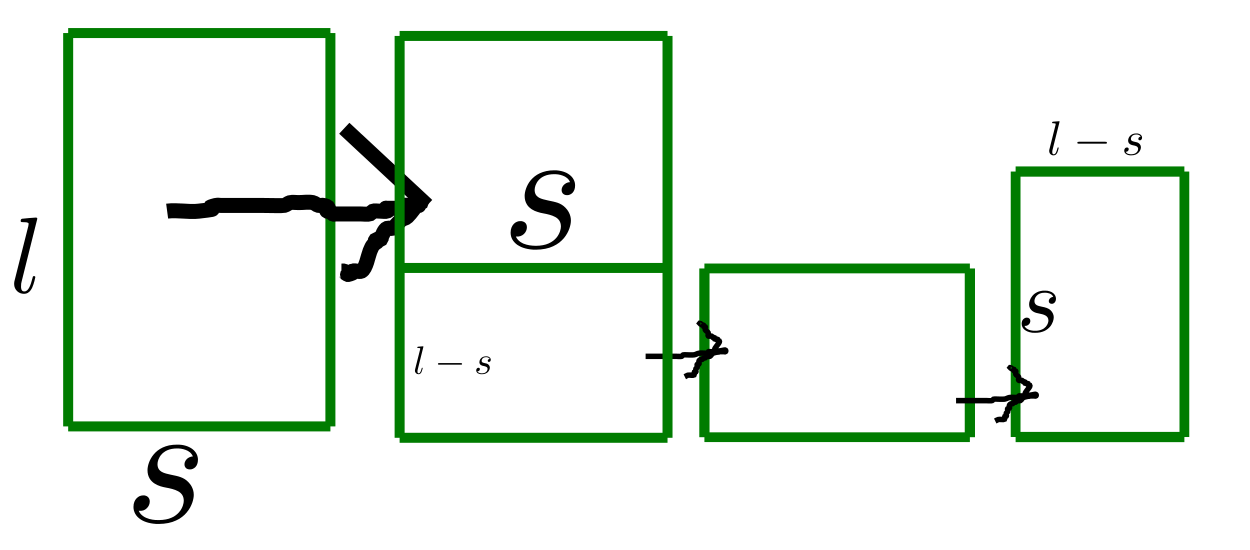
\includegraphics[scale=0.15]{chop-arrow-labeled2}

\begin{figure}


\caption{Equation of Golden Rectangle}


\[
\frac{l}{s}=\frac{s}{l-s}
\]
\end{figure}



\lyxframeend{}


\lyxframeend{}\lyxframe{Golden Equation}

\begin{eqnarray*}
\frac{l}{s} & = & \frac{s}{l-s}\\
l\,\left(l-s\right) & = & s^{2}\\
l^{2}-ls & = & s^{2}\\
\frac{l^{2}-ls}{s^{2}} & = & \frac{s^{2}}{s^{2}}\\
\left(\frac{l}{s}\right)^{2}-\frac{l}{s} & = & 1
\end{eqnarray*}


Now let $\phi$ (phi) be $\frac{l}{s}$ the ratio of the long to the
short sides. Then this equation is:

\begin{eqnarray*}
\phi^{2}-\phi & = & 1\\
\phi^{2}-\phi-1 & = & 0
\end{eqnarray*}



\lyxframeend{}


\lyxframeend{}\lyxframe{Golden Equation roots.}

\[
\phi^{2}-\phi-1=0
\]


If we apply the quadratic formula to this equation, we find:

\[
\phi=\frac{1\pm\sqrt{1+4}}{2}=\frac{1\pm\sqrt{5}}{2}
\]


The negative root we can lay aside for the moment, as a distance or
a ratio of distances can not be negative. The positive root is:

\[
\frac{1+\sqrt{5}}{2}=1.618033989...
\]


This is the Golden Ratio, which often crops up uncannily in mathematics,
nature, art, and the occult.


\lyxframeend{}


\lyxframeend{}\lyxframe{Golden ratio conjugate}

Let us consider the other root $\frac{1-\sqrt{5}}{2}$. This is a
negative number, and the ancient Greeks did to believe in negative
numbers, so we will consider its negative, $\Phi=-\frac{1-\sqrt{5}}{2}$.
It is called the Golden ratio conjugate. Consider $\phi\,\Phi$:

\begin{eqnarray*}
\phi\,\Phi & = & \frac{1+\sqrt{5}}{2}\,\left(-1\right)\,\frac{1-\sqrt{5}}{2}\\
 & = & \left(-1\right)\,\frac{1-5}{4}\\
 & = & 1
\end{eqnarray*}
\textrm{ So $\phi$ and $\Phi$ are reciprocals. To divide by one,
multiply by the other.}


\lyxframeend{}


\lyxframeend{}\lyxframe{Analyzing the Golden Triangle}


\column{15cm}

abc


\end{document}
